\chapter{Konzeption}
\label{ch:intro}
In diesem Kapitel wird das Konzept des Filmes erklärt. Hierzu gehören alle grundsätzlichen Entscheidungen, wie der Inhalt des Dargestellten, die Darstellungsweise und die Zielgruppe.

\section{Zielgruppe}
\label{sec:konzept:zielgruppe}

% \graffito{Note: The content of this chapter is just some dummy text. It is not a real language.}

Als Zielgruppe wurden Kunden anvisiert, für die es in Frage kommt die Drohne einzusetzen. Dabei soll diese Zielgruppe nach dem Film wissen, wie die Drohne konkret eingesetzt wird, welche Schritte hierfür nötig sind und mit welchem Aufwand ein Einsatz einhergeht. Solche Kunden sind beispielsweise Sea-Watch, Sea-Eye und Resqship. Diese Organisationen haben sich zur Aufgabe gemacht Flüchtlinge, die über das Mittelmeer nach Europa kommen und in Seenot geraten, zu retten. Da diese Rettungsorganisationen nicht die Mittel für Hubschrauberflüge haben, sondern nur mit einem Schiff unterwegs sind, ist der Suchradius stark eingeschränkt. Daher ist das Ziel der Drohne diesen Suchradius zu erweitern. \\
Sekundär sollen auch an dem Projekt Interessierte und potenzielle Teammitglieder eine Zielgruppe sein. Dies hatte zur Folge, dass wenige Informationen noch ergänzend eingefügt wurden, um einem interessierten Zuschauer alle nötigen Informationen zu bieten.\\
Weil der Zielgruppe, die die Drohne einsetzt, wichtig ist, dass die Drohne nicht nur ein Konzept ist, sondern schon funktionsfähig im Einsatz ist, wurde die Entscheidung getroffen den Film auf schon vorhandenem Filmmaterial aufzubauen. Somit wird gezeigt, dass die Drohne schon gebaut wurde und funktionsfähig eingesetzt wird. Die Funktionsweise ist jedoch schwer mit Filmmaterial darstellbar, weswegen ein Teil des Filmes mit Computeranimationen ergänzt wird. Beispiele für diese Erklärungen sind der Flugpfad des Flugzeugs, oder das Sichtfeld. Außerdem ist das Filmen einer realen Drohne im Flug nur schwer durchzuführen.

\section{Struktur} % Outline
\label{sec:konzept:outline}

Es wurde in Rücksprache mit dem SearchWing-Team definiert, dass folgende sechs Punkte im Film in dieser Reihenfolge erscheinen sollen.

\begin{itemize}
\setlength\itemsep{0pt}
\item{Flugplanerstellung}
\item{Montage}
\item{Start}
\item{Flug}
\item{Landung}
\item{Auswertung}
\end{itemize}
\noindent
Bei der Flugplanerstellung wird der Bereich mithilfe eines Tablets definiert, in dem die Drohne nach Schiffbrüchigen suchen soll. Bei der Montage wird gezeigt, wie die Tragflächen an den Rumpf angebracht werden, da mit demontierten Teilen das Gerät leichter zu transportieren ist. Anschließend wird der Start aus der Hand gezeigt. Im Flug wird dargestellt, wie die Aufnahme der Bilder funktioniert. Danach wird eine Landung der Drohne im Wasser dargestellt. Der letzte Vorgang, der behandelt wird, ist das Betrachten und Auswerten der erstellten Bilder am Laptop.\\
Zusätzlich zu diesen sechs inhaltlichen Punkten wurden ein Intro und ein Outro mit ähnlicher Bildsprache eingefügt. Somit bekommt der Film einen angenehmen Rahmen.\\
Wie unter \autoref{sec:konzept:zielgruppe} beschrieben, wurde vorhandenes Filmmaterial benutzt. Da diese Sequenz bereits geschnittenes Material von einem Rundfunkbeitrag war, standen nur relativ kurze Ausschnitte von Szenen zur Verfügung. 
Um innerhalb dieser kurzen Zeit trotzdem alle gewünschten Informationen zu vermitteln, wurde entschieden, nicht mit einem Sprecher zu arbeiten, sondern mit Texteinblendungen. Diese benötigen deutlich weniger Zeit, da hier nur Stichpunkte gelesen werden und keine vollständigen Sätze von einem Sprecher vorgetragen werden.
Später wurde festgelegt, dass am Ende des Filmes, im Kapitel ``Auswertung'', ein Rettungsfloß eingefügt werden soll, damit der Rezipient eine Erfolgreiche Story vermittelt bekommt.\\
Die Kapitel ``Flug'' und ``Landung'' -- abgesehen von Intro und Outro -- sind die Teile des Filmes, welche mit Computeranimationen entstanden sind. Hierbei wurde entschieden, dass ein möglichst realistischer Look angestrebt wird, damit sich diese Teile möglichst gut in das Filmmaterial einfügen.

\section{Storyboard} % Layout
\label{sec:konzept:animatic}

Der Flug wurde in einem Storyboard grob dargestellt (siehe \autoref{animatic}). In diesem Fall wurden mit einfachen 3D-Modellen pro Kameraeinstellung ein Bild erstellt. Hierzu wurde das Modell eines Segelbootes importiert und ein stark vereinfachtes Modell eines Flugzeuges eingefügt. Anschließend konnten zu den Arten der Information passende Kameraeinstellungen definiert werden. So wird beispielsweise beim Steigflug des Flugzeuges die Höhe eingeblendet, oder bei der Fluggeschwindigkeit das Flugzeug etwas weiter von Hinten gezeigt. \\
Ebenso wurde bei den Kameraeinstellungen darauf geachtet, dass stets eine Referenz aus dem vorherigen Schnitt zu sehen ist. Folglich ist am Anfang der Flugeinstellung das Segelboot zu sehen, genauso auch am Ende des Fluges.\\
Für Intro und Outro wurden ein Flug über das Meer und ein vergleichsweise kleiner Rettender gewählt, um sowohl die Problematik als auch den Erfolg mithilfe der Drohne zu verstärken.
Diese Bilder wurden in den ersten Zusammenschnitt des Filmmaterials eingefügt. Damit wurde ein erster Eindruck erschaffen, ob der Film schlüssig ist und alle nötigen Informationen transportiert werden. Später wurde die Reihenfolge der Informationen und der dazugehörigen Einstellungen geändert, um eine schlüssigere Reihenfolge zu realisieren.

\begin{figure}[H]
\centering
\begin{longtable}{cc}
\subfloat[Start vom Boot]{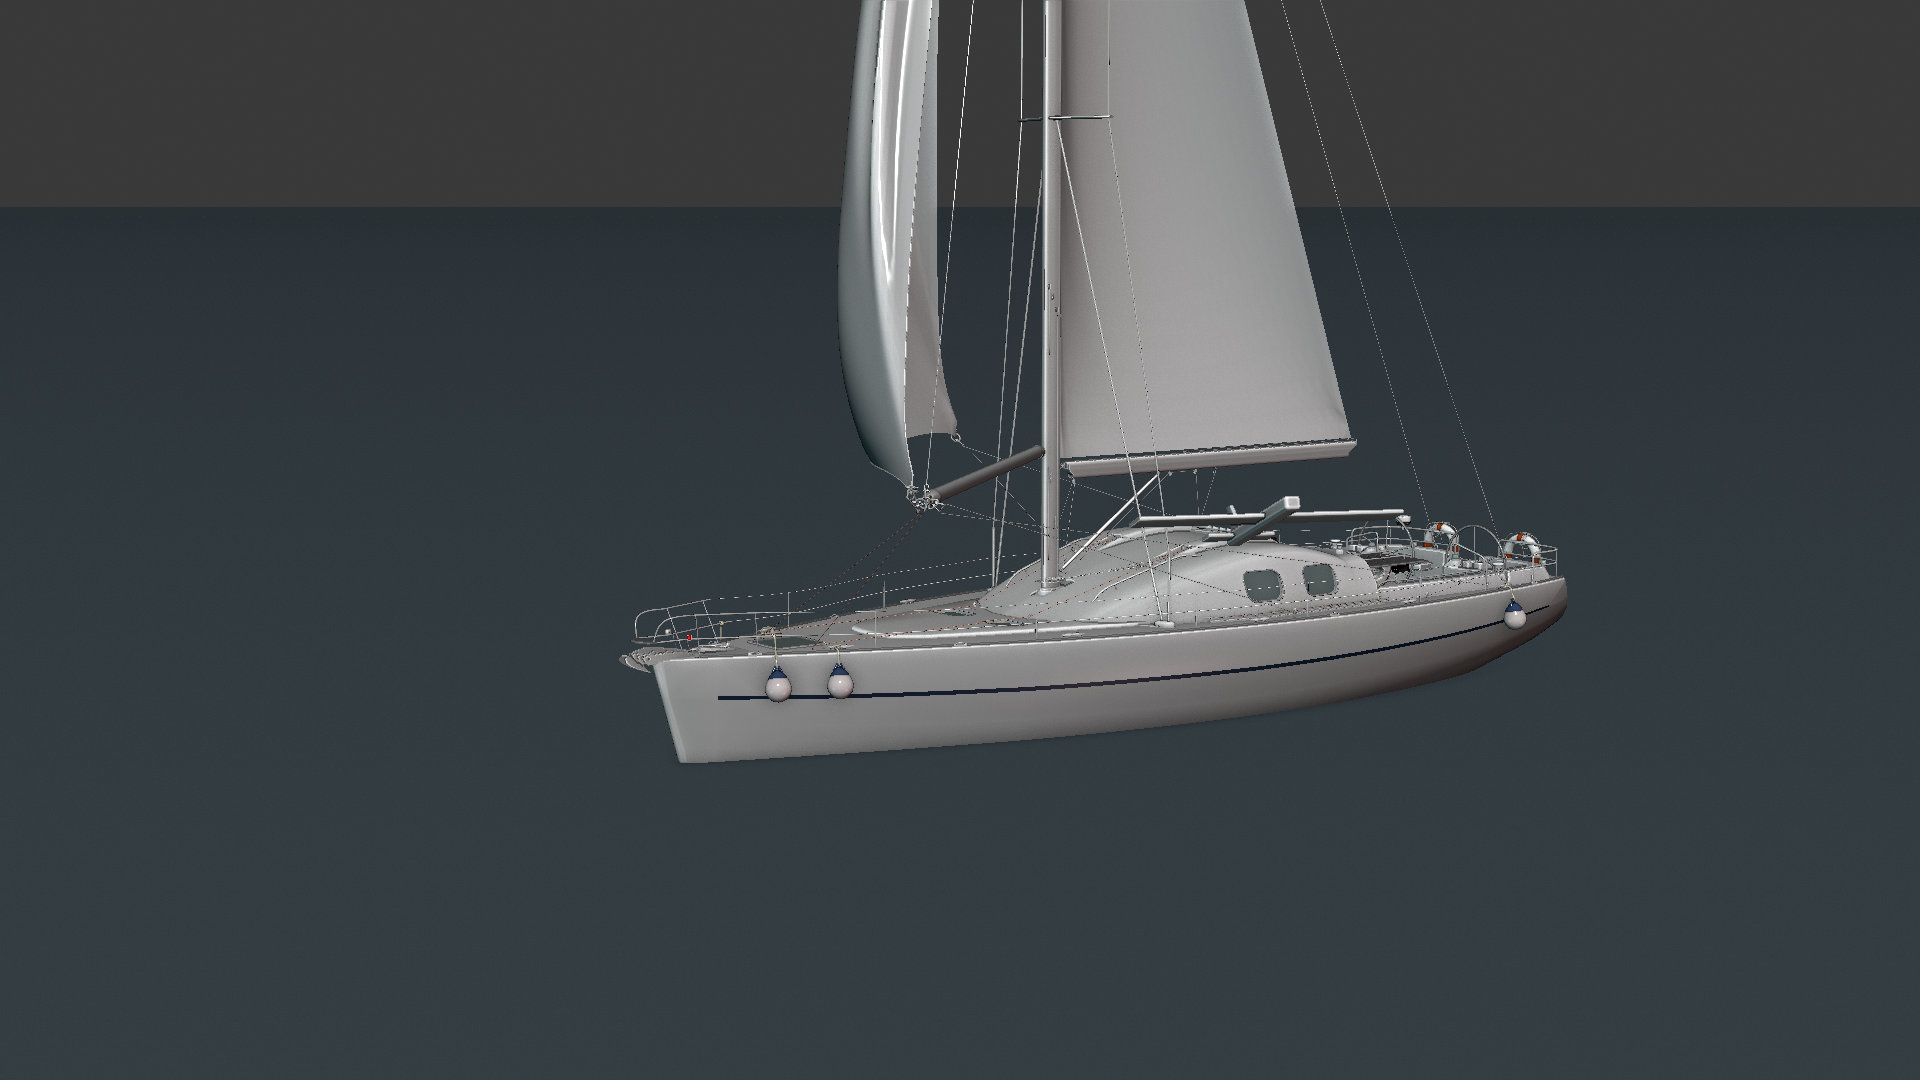
\includegraphics[width=0.5\textwidth]{gfx/pre/0058.jpg}} &
\subfloat[Steigflug]{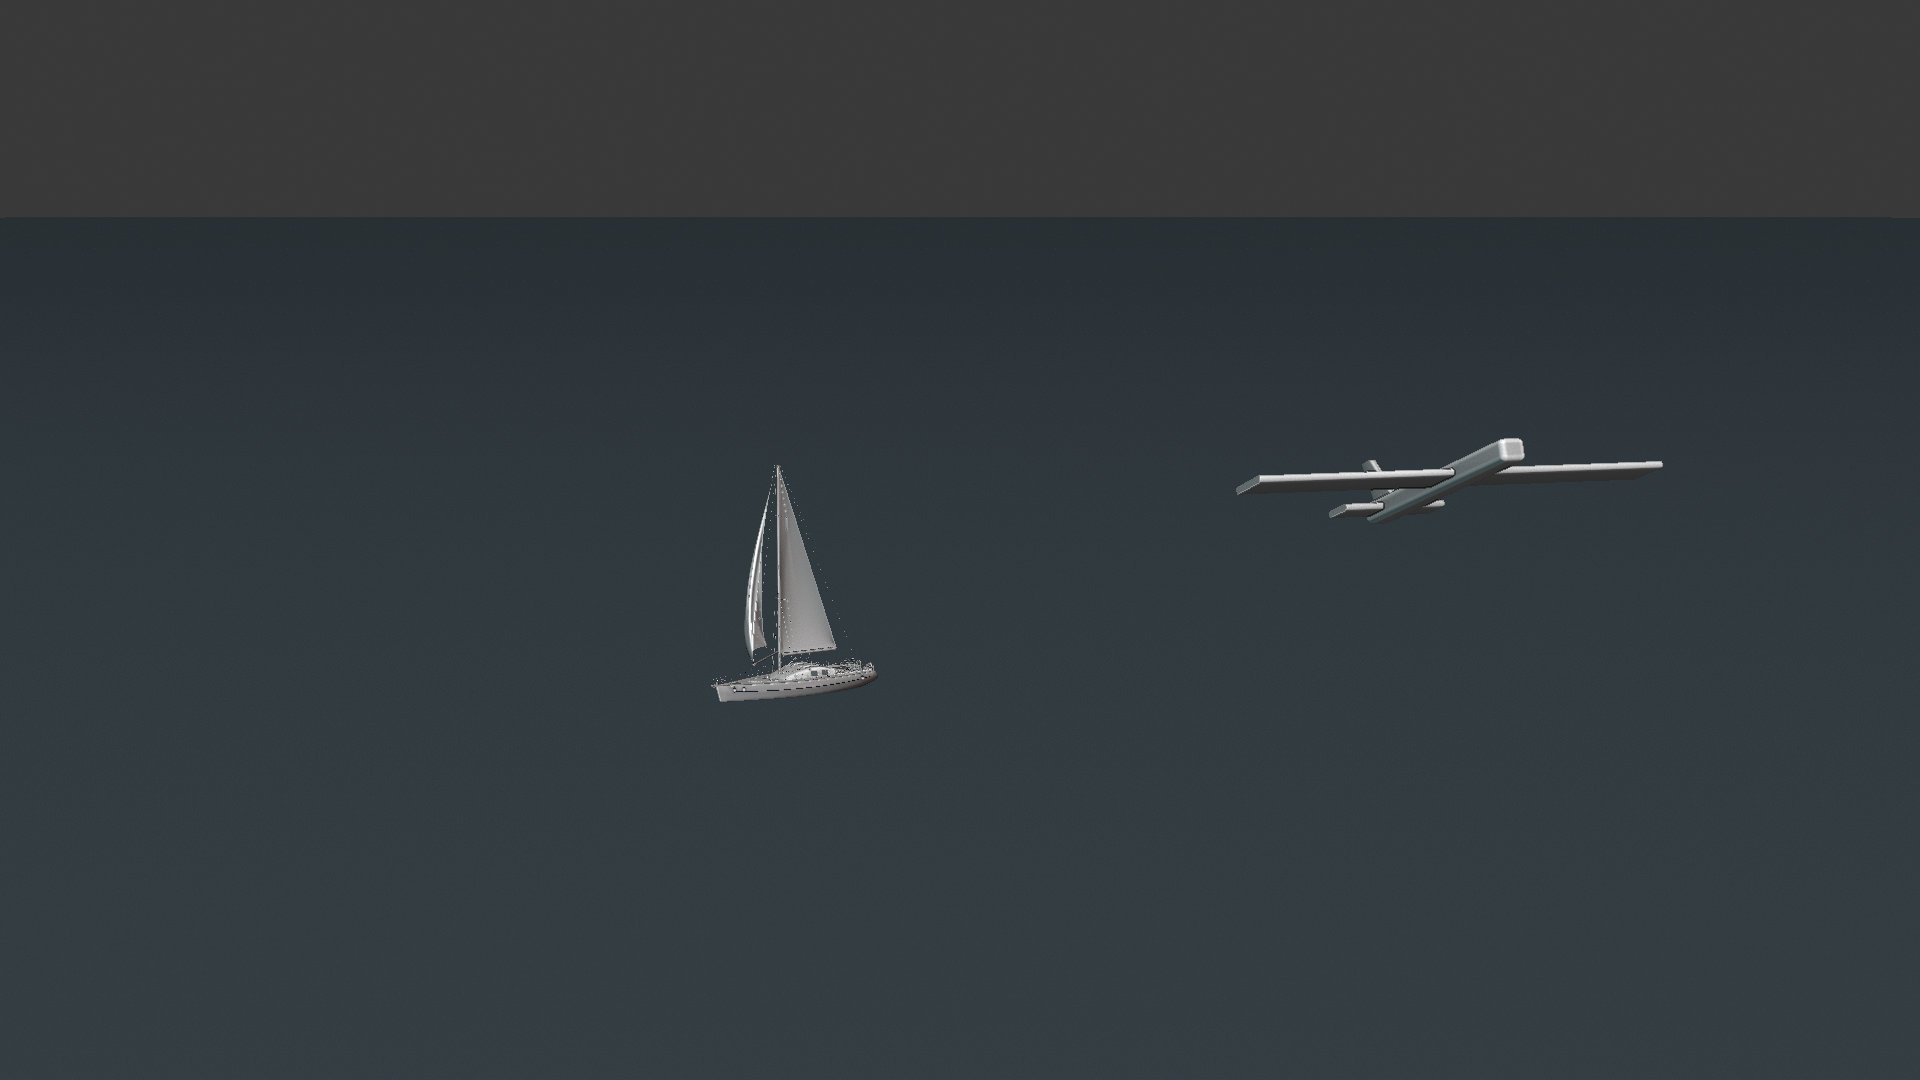
\includegraphics[width=0.5\textwidth]{gfx/pre/0059.jpg}} \\
\subfloat[Fluggeschwindigkeit]{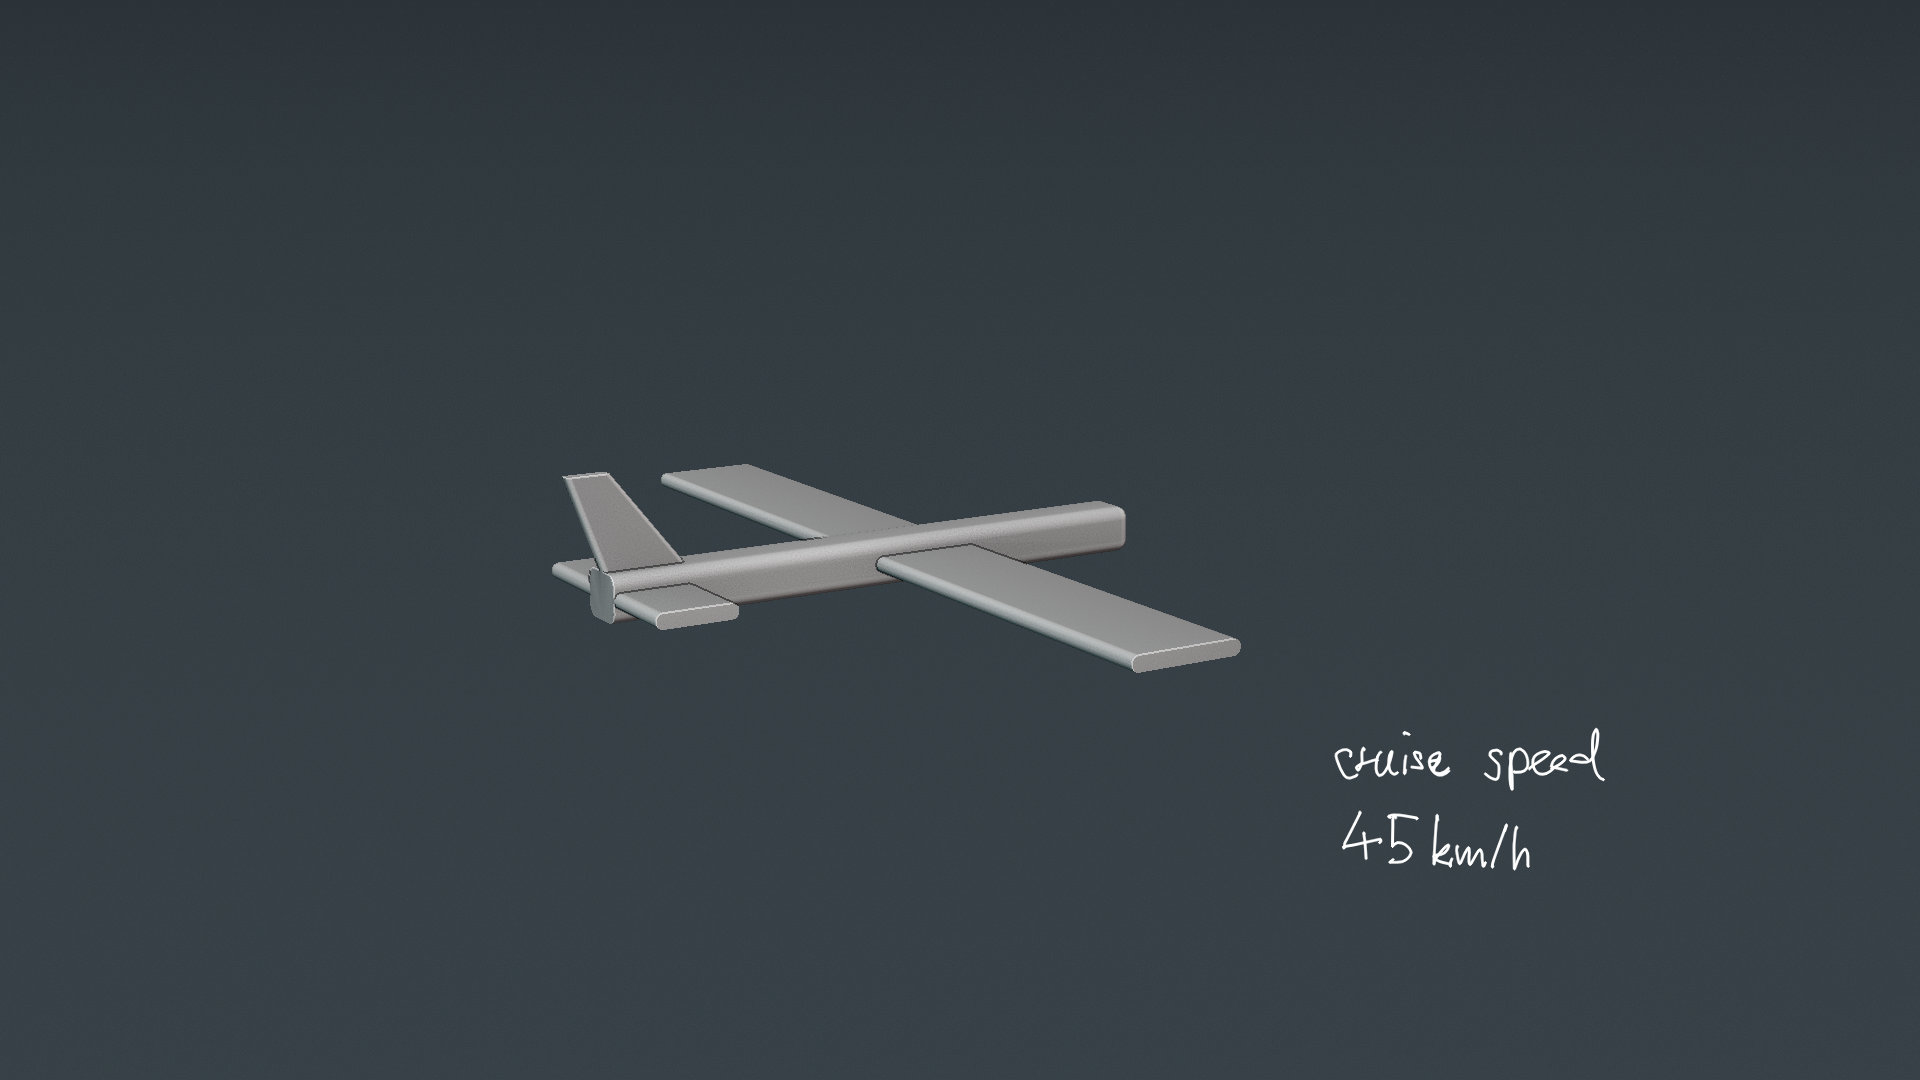
\includegraphics[width=0.5\textwidth]{gfx/pre/0180.jpg}} &
\subfloat[maximalgeschwindigkeit]{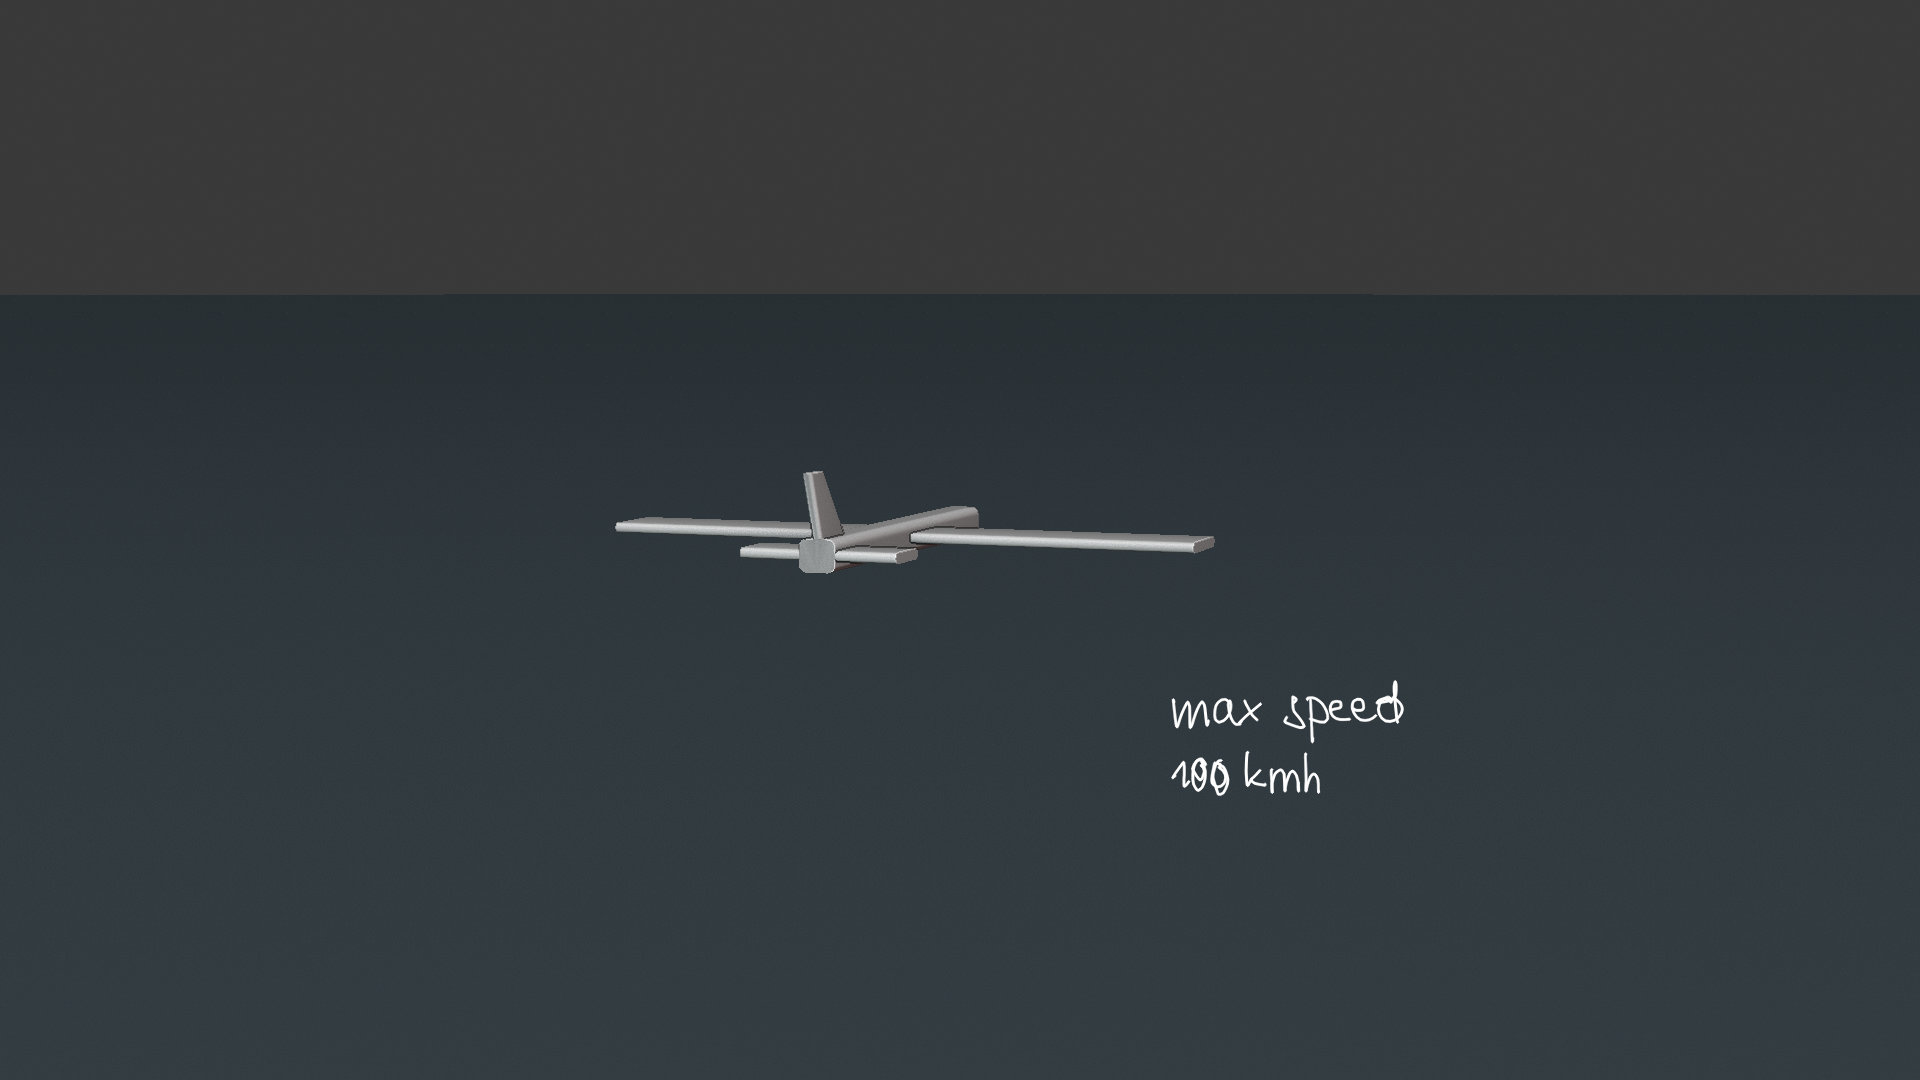
\includegraphics[width=0.5\textwidth]{gfx/pre/0239.jpg}} \\
\subfloat[Flughöhe]{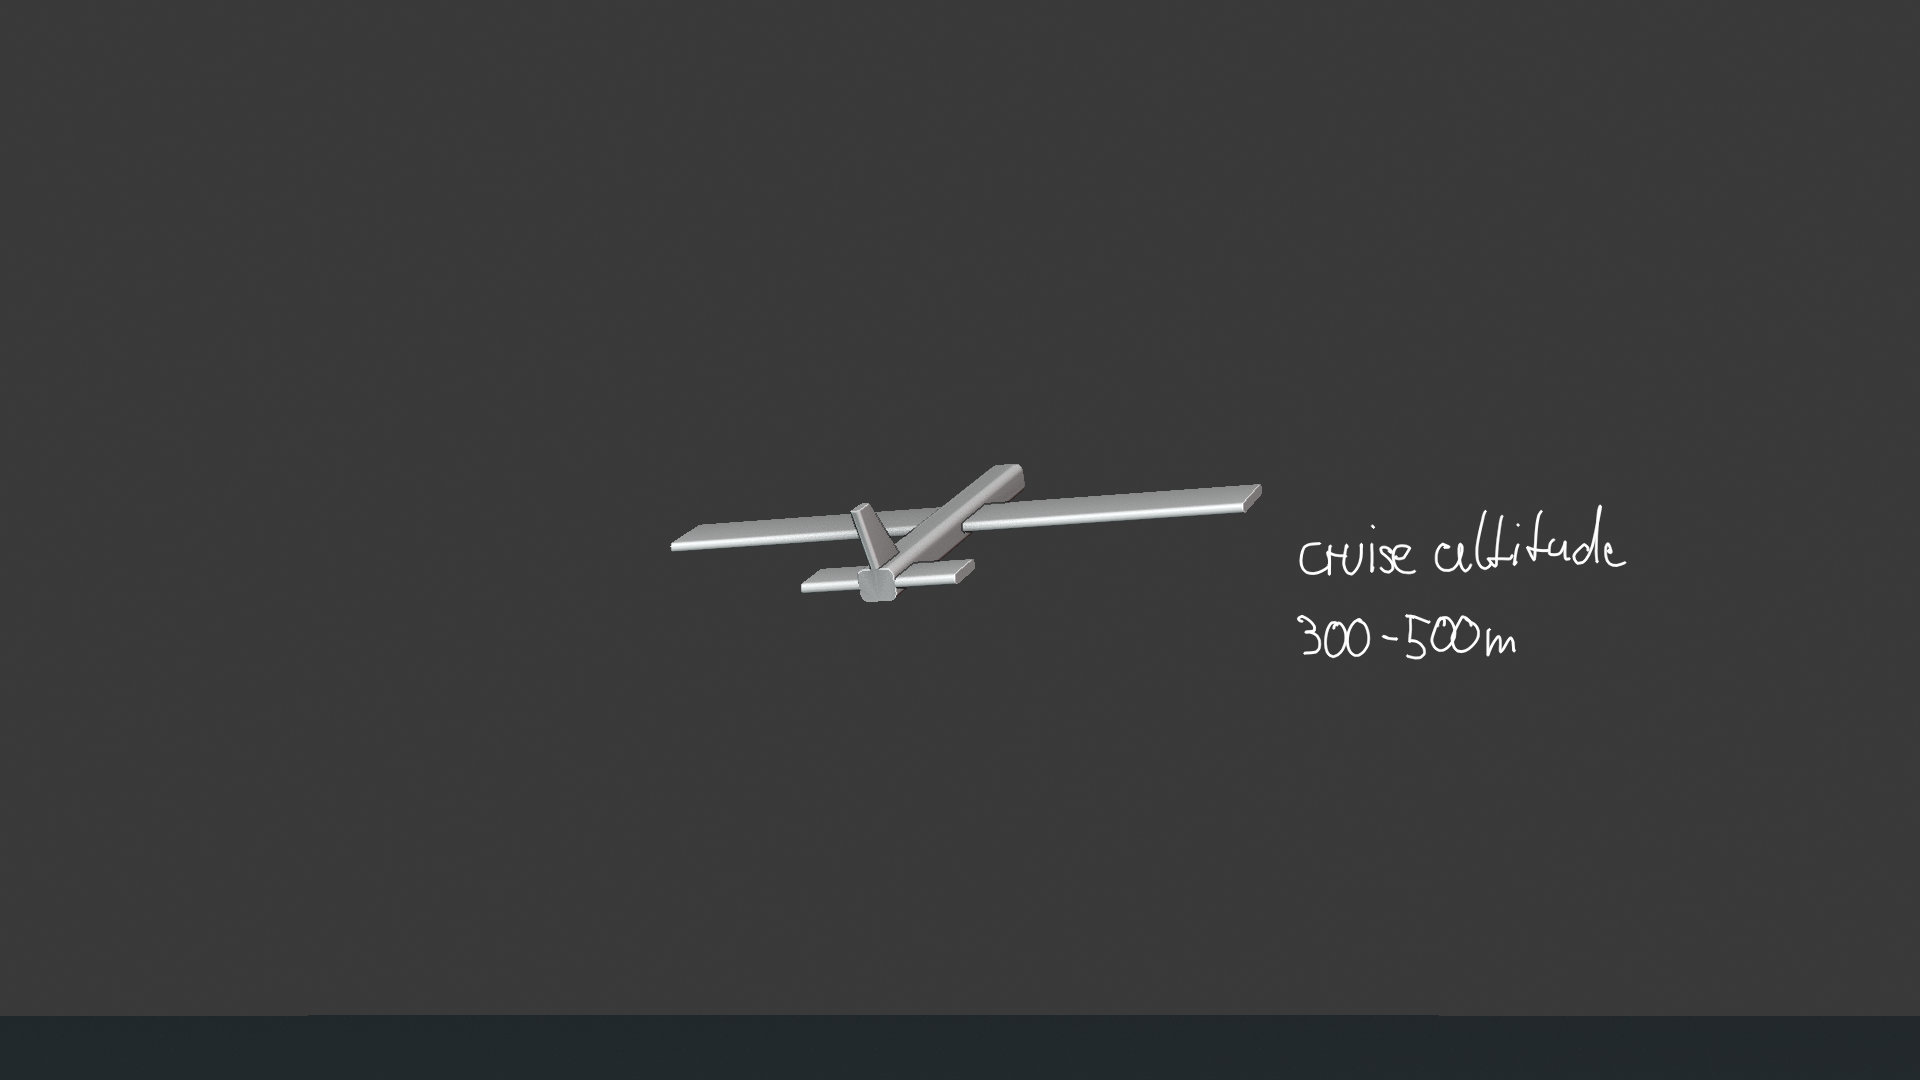
\includegraphics[width=0.5\textwidth]{gfx/pre/0321.jpg}} &
\subfloat[Sichtfeld]{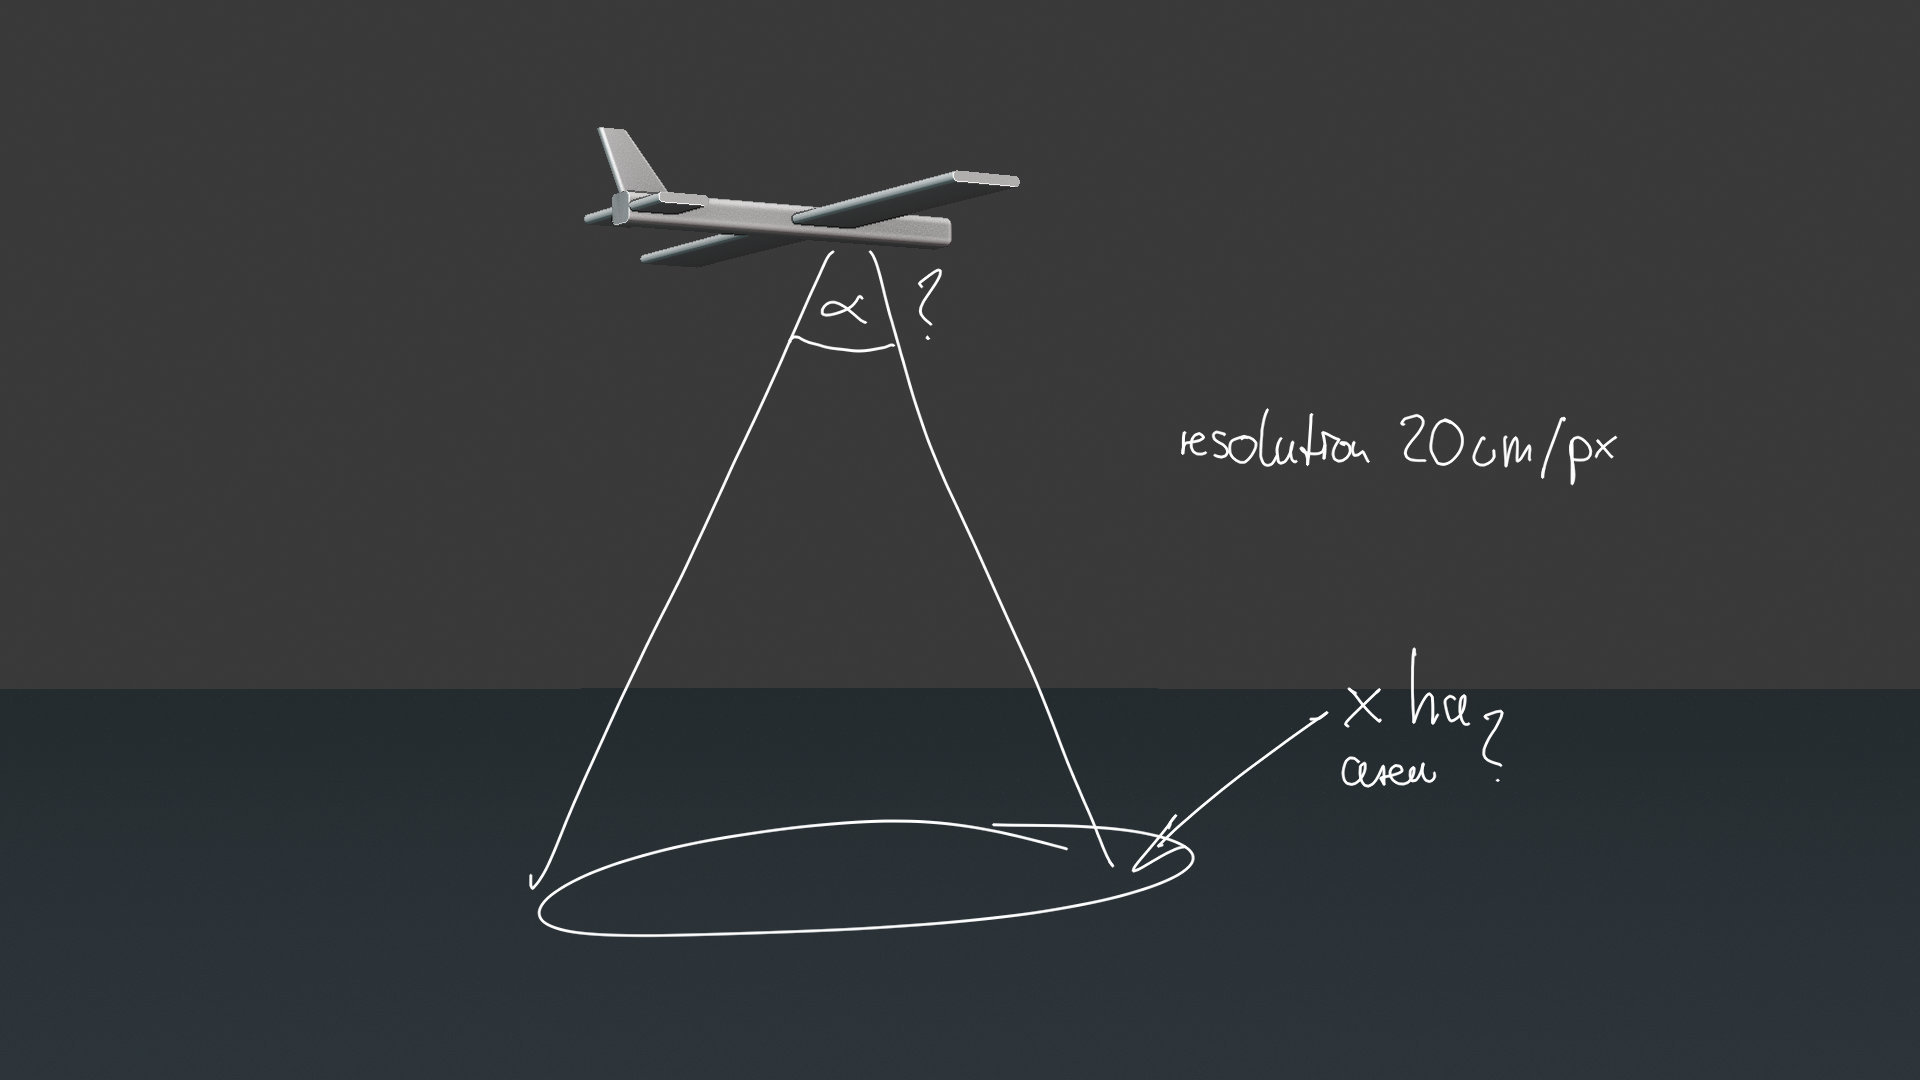
\includegraphics[width=0.5\textwidth]{gfx/pre/0362.jpg}} \\
\subfloat[Ansicht von oben]{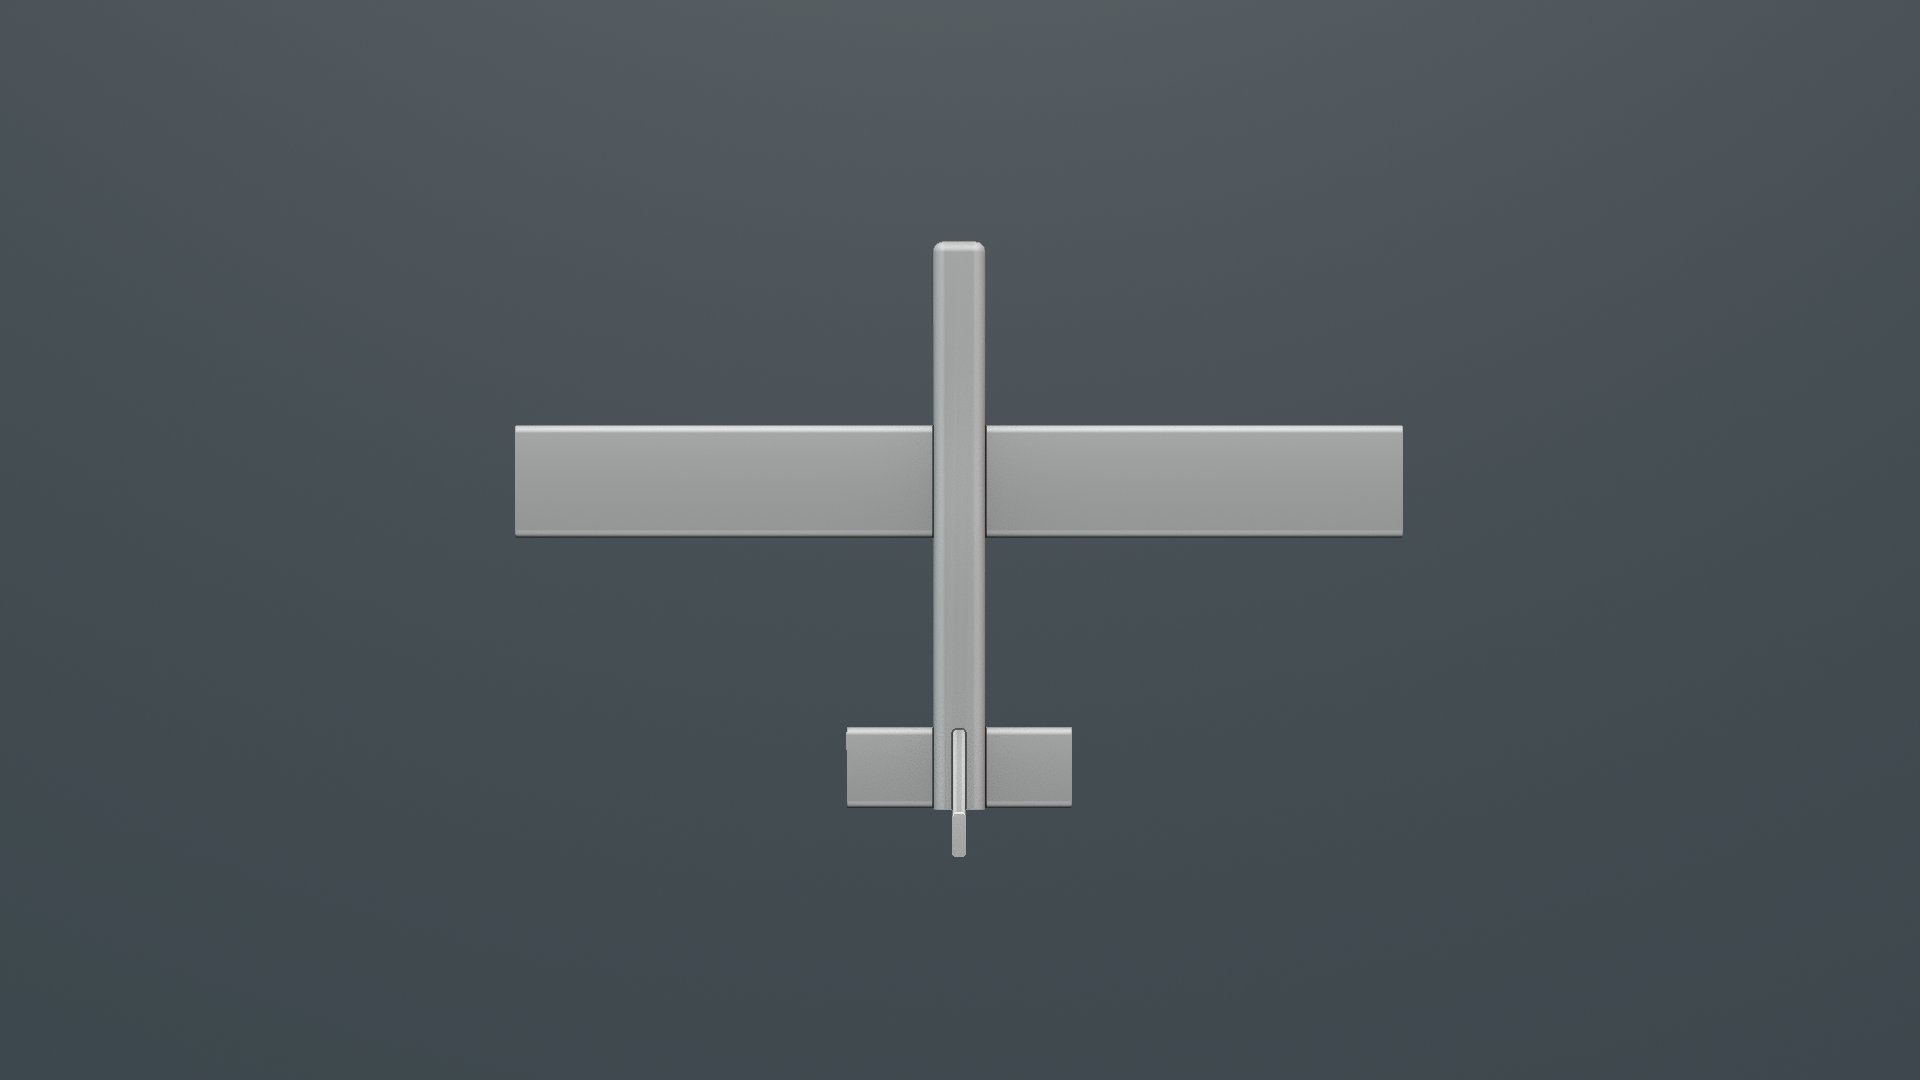
\includegraphics[width=0.5\textwidth]{gfx/pre/0442.jpg}} &
\subfloat[Darstellung des Flugpfades]{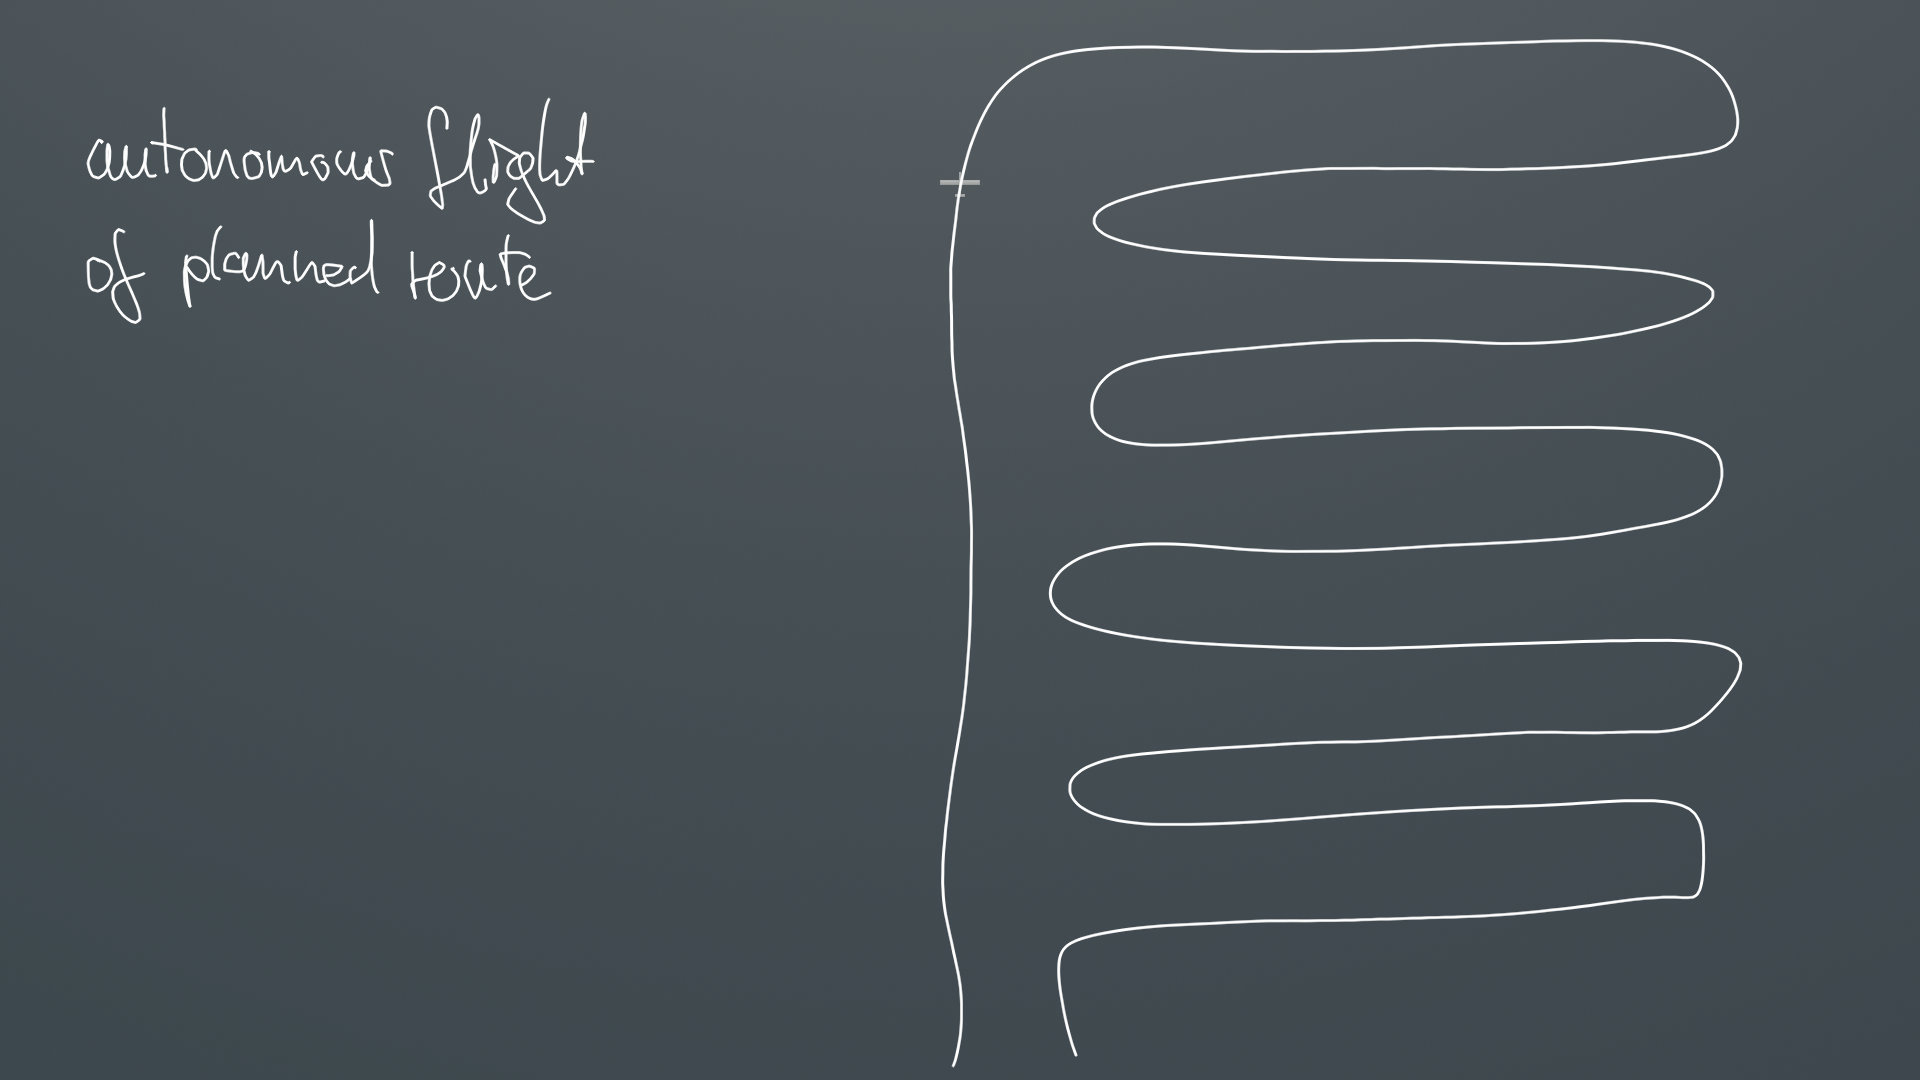
\includegraphics[width=0.5\textwidth]{gfx/pre/0483.jpg}} \\
\subfloat[Reichweite]{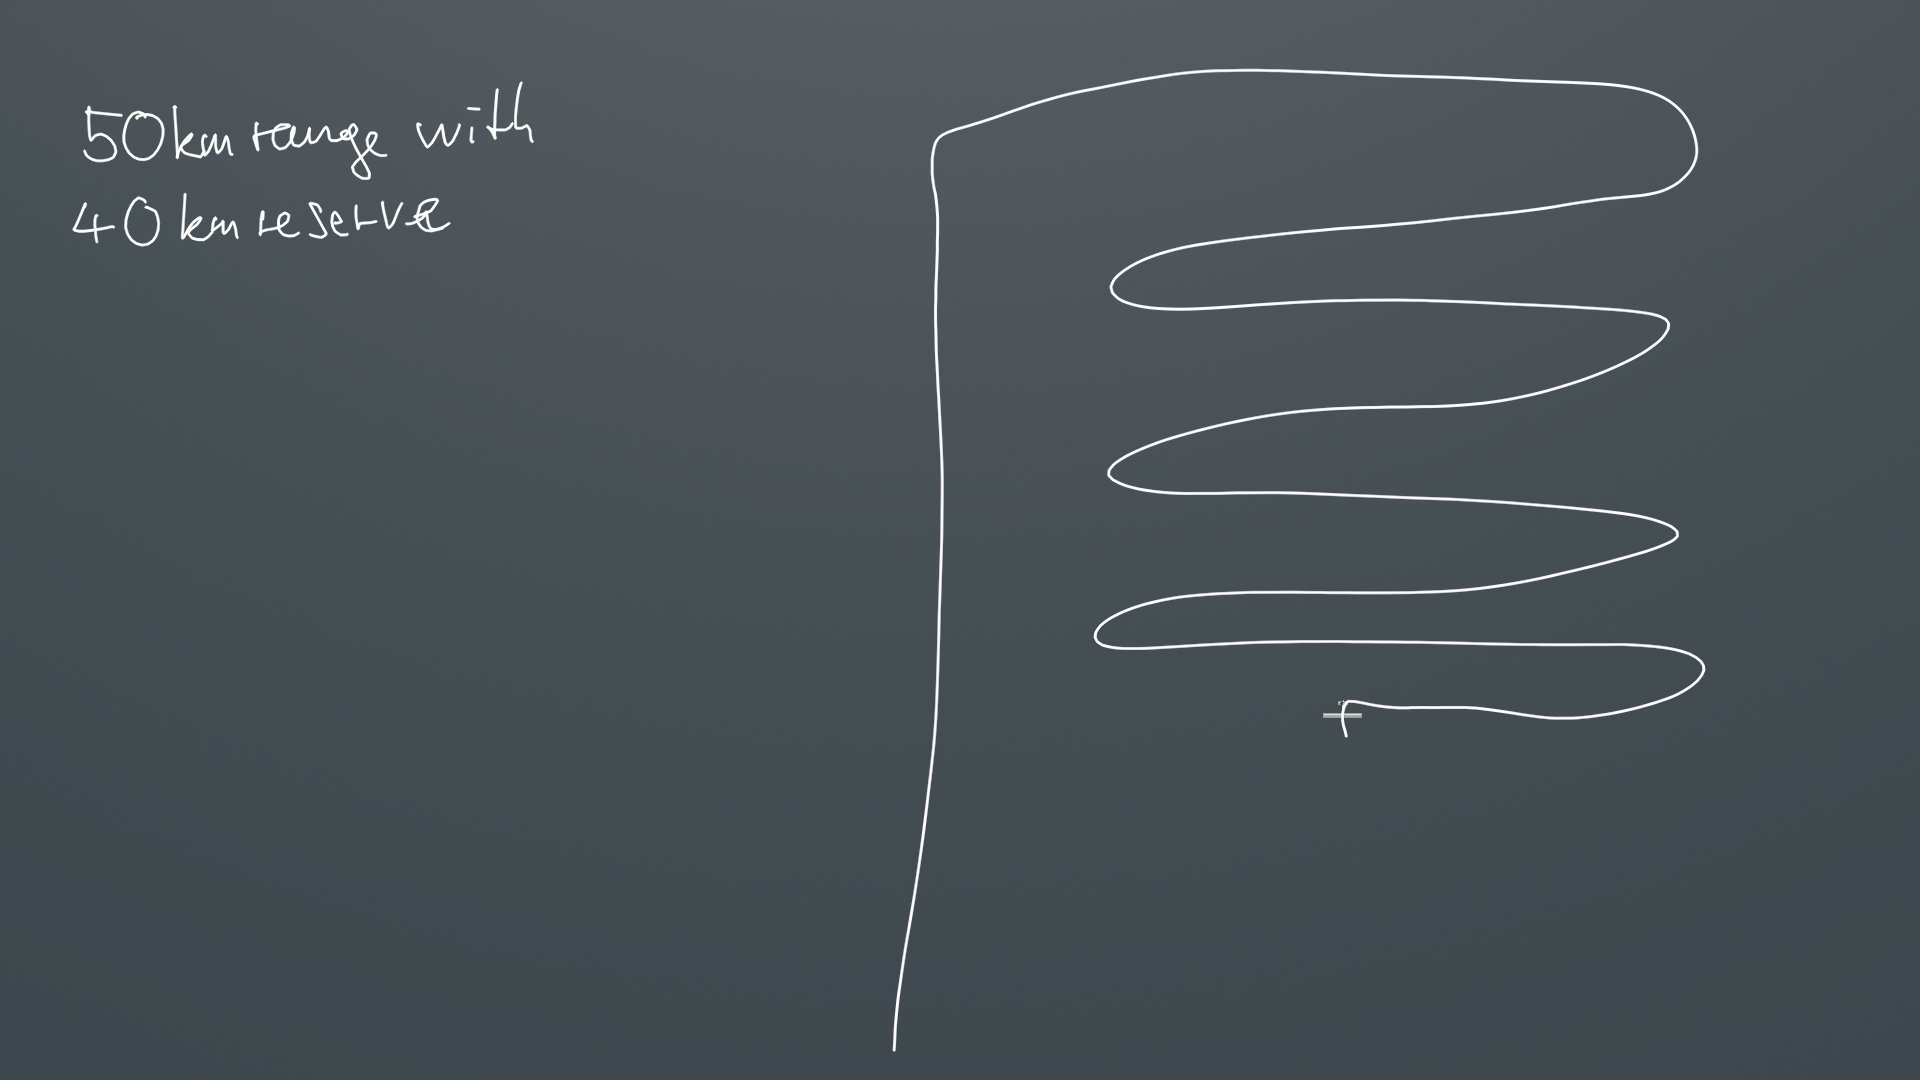
\includegraphics[width=0.5\textwidth]{gfx/pre/0565.jpg}} &
\subfloat[Rückkehr zum Boot]{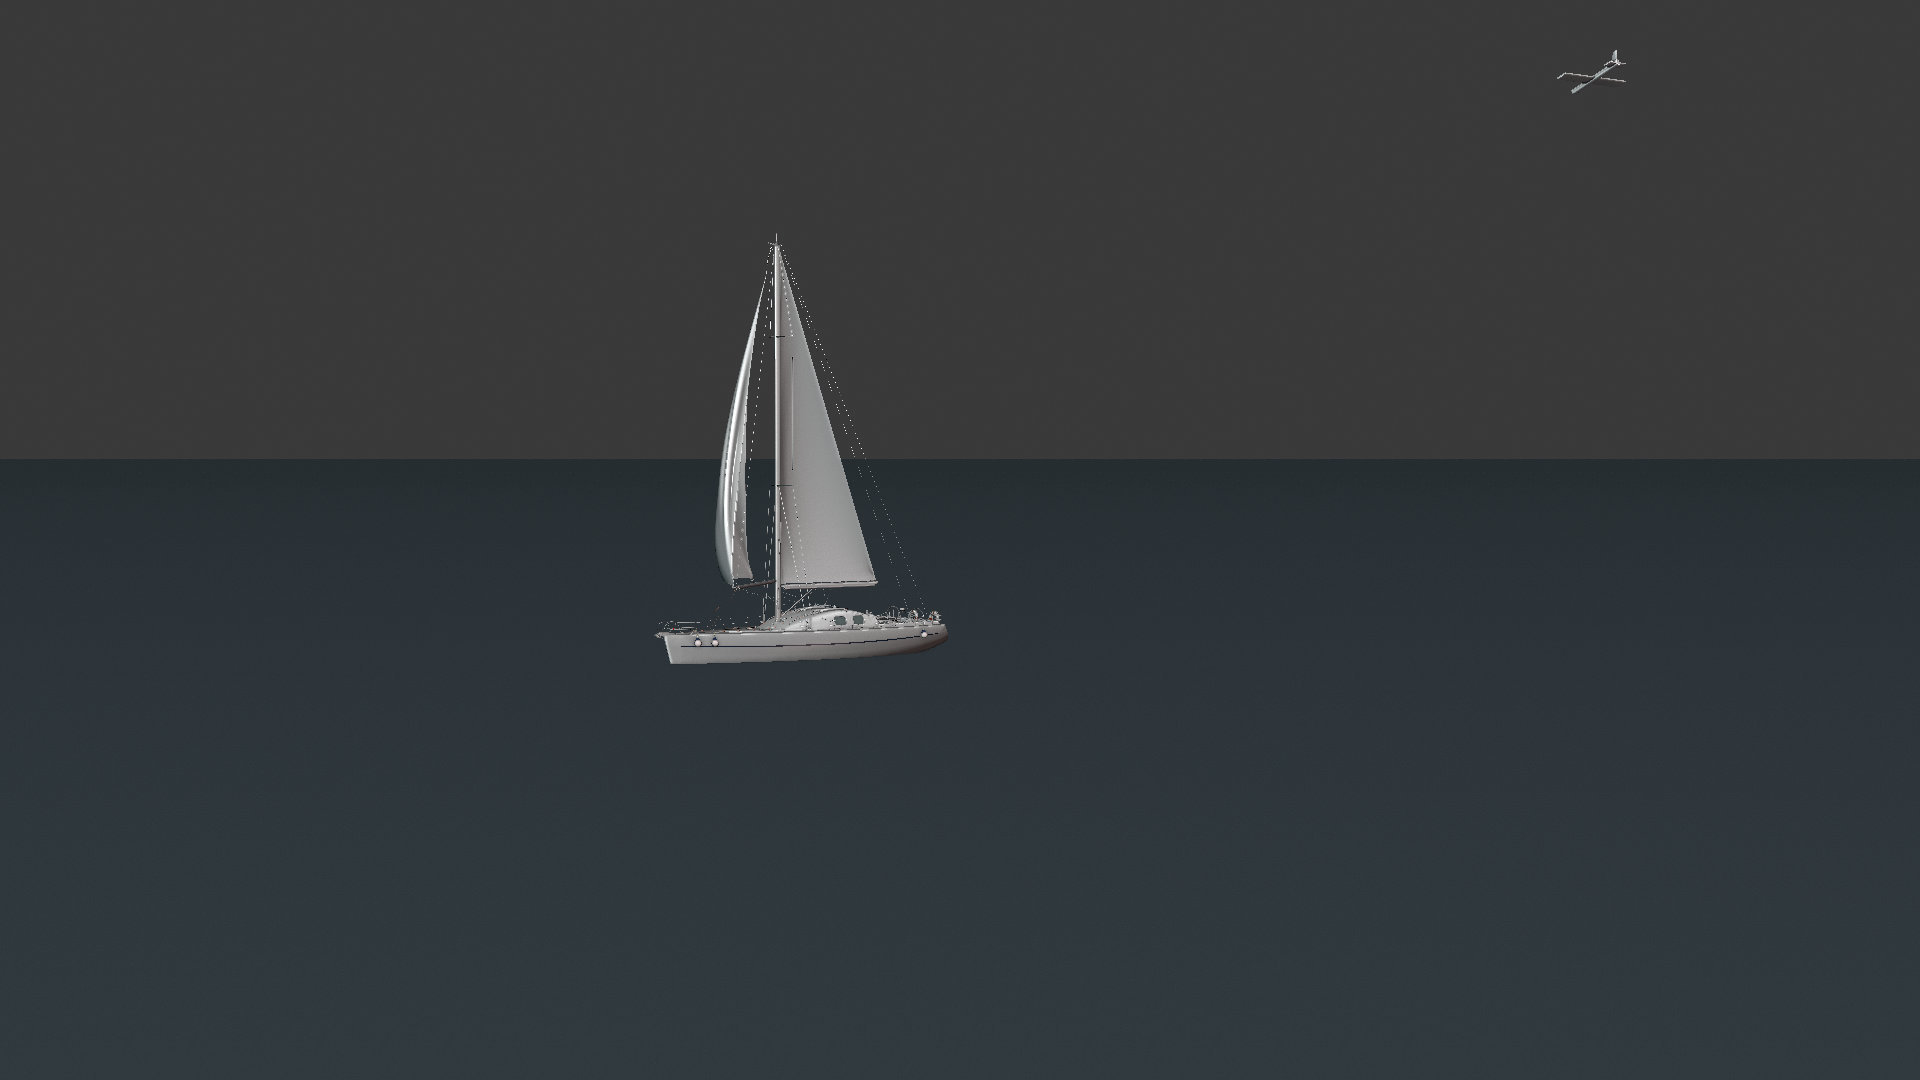
\includegraphics[width=0.5\textwidth]{gfx/pre/0688.jpg}}\\

\end{longtable}
\caption{Einzelbilder des Storyboards}
\label{animatic}
\end{figure}
%

% \begin{figure}[H] \ContinuedFloat
% \raggedleft
% \begin{longtable}{ll}


% \end{longtable}
% \caption{Einzelbilder des Storyboards}
% \label{animatic}
% \end{figure}

